\documentclass{beamer}

\usepackage{tikz}
\usetikzlibrary{patterns}
\usetikzlibrary{calc}
\usetikzlibrary{shapes, arrows, positioning}

\usepackage{tabularray}
\UseTblrLibrary{booktabs}
\DefTblrTemplate{contfoot-text}{normal}{\lang{(Continued on next page)}{(Continua na próxima página)}} 
\SetTblrTemplate{contfoot-text}{normal} 
\DefTblrTemplate{conthead-text}{normal}{\lang{(continued)}{(continuação)}} 
\SetTblrTemplate{conthead-text}{normal}

\usepackage{enumitem}
\definecolor{ifscgreen}{RGB}{50,93,61}

\setlist[enumerate,1]{label=\colorbox{ifscgreen}{\textcolor{white}{\arabic*}}\quad, leftmargin=*}
\setlist[enumerate,2]{label=\colorbox{ifscgreen!70}{\textcolor{white}{\arabic{enumi}.\arabic*}}\quad, leftmargin=*}
\setlist[enumerate,3]{label=\colorbox{ifscgreen!40}{\textcolor{white}{\arabic{enumi}.\arabic{enumii}.\arabic*}}\quad, leftmargin=*}
% ------------------------------
% Codificação e idioma
% ------------------------------
% \usepackage[utf8]{inputenc}
\usepackage[T1]{fontenc}
\usepackage[brazil]{babel}

% ------------------------------
% Matemática e símbolos
% ------------------------------
\usepackage{amsmath}

% ------------------------------
% Gráficos e figuras
% ------------------------------
\usepackage{graphicx}
\usepackage{subfigure}

% ------------------------------
% Cores, URL e hiperlinks
% ------------------------------
\usepackage{url,color}
\usepackage{hyperref}
\hypersetup{
  pdfstartview={Fit},
  pdftitle={\@title},
  pdfsubject={Engenharia de Telecomunicacoes - IFSC},
  pdfauthor={\@author}
}

% ------------------------------
% Listagens e pseudocódigo
% ------------------------------
\usepackage[
plainruled,
noline
]{algorithm2e}

% ------------------------------
% Bibliografia
% ------------------------------
\usepackage[backend=biber,style=numeric,citestyle=ieee]{biblatex}
\addbibresource{references.bib}
\setbeamertemplate{bibliography item}{\insertbiblabel}

% ------------------------------
% Outros pacotes
% ------------------------------
\usepackage{ifsc} % (pacote personalizado, ok manter)

% ------------------------------
% Macros e comandos personalizados
% ------------------------------
\newcommand{\tab}[1]{\hspace{.2\textwidth}\rlap{#1}}

\newcommand{\DAY}{\the\day}
\newcommand{\MONTH}{%
  \ifcase\the\month
  \or Janeiro%
  \or Fevereiro%
  \or Março%
  \or Abril%
  \or Maio%
  \or Junho%
  \or Julho%
  \or Agosto%
  \or Setembro%
  \or Outubro%
  \or Novembro%
  \or Dezembro%
  \fi}
\newcommand{\YEAR}{\the\year}

% ------------------------------
% Dados do título
% ------------------------------
\title{PRG203402 - Lógica de Programação:}
\subtitle{\LARGE Estruturas de decisão e repetição}
\author{João Cláudio Elsen Barcellos}
\date{\scriptsize \DAY~de \MONTH~de \YEAR}
\institute{
  Engenheiro Eletricista\\
  Formado na Universidade Federal de Santa Catarina\\
  campus Florianópolis\\
  \url{joaoclaudiobarcellos@gmail.com}
}

% ------------------------------
% Customização das seções no Beamer
% ------------------------------
\def\sectionname{}
\def\insertsectionnumber{}
\def\subsectionname{}
\def\insertsubsectionnumber{}

\AtBeginSection[]{
  \begin{frame}
      \vfill
      \centering
      \begin{beamercolorbox}[sep=8pt,center,shadow=true,rounded=true]{title}
          \usebeamerfont{title}\insertsectionhead\par%
      \end{beamercolorbox}
      \vfill
  \end{frame}
}

\setbeamertemplate{caption}[numbered]

% ------------------------------
% Controle de idioma
% ------------------------------
\usepackage{ifthen}
\newboolean{english}
\setboolean{english}{false} % true = inglês, false = português

% Configuração de idioma e títulos
\ifthenelse{\boolean{english}}{
  \usepackage[english]{babel}
  \renewcommand{\figurename}{Figure}
  \renewcommand{\tablename}{Table}
  \SetAlgorithmName{Algorithm}{}{}
  
  \SetKwInput{KwData}{Input}
  \SetKwInput{KwResult}{Output}
  \SetKwIF{If}{ElseIf}{Else}{if}{then}{else if}{else}{end if}
  \SetKwFor{While}{while}{do}{end while}
  \SetKwFor{For}{for}{do}{end for}
  \SetKw{Return}{return}
}{
  \usepackage[brazil]{babel}
  \renewcommand{\figurename}{Figura}
  \renewcommand{\tablename}{Tabela}
  \SetAlgorithmName{Algoritmo}{}{}
  
  \SetKwInput{KwData}{Entrada}
  \SetKwInput{KwResult}{Saída}
  \SetKwIF{If}{ElseIf}{Else}{se}{então}{senão se}{senão}{fim}
  \SetKwFor{While}{enquanto}{faça}{fim}
  \SetKwFor{For}{para}{faça}{fim}
  \SetKw{Return}{retorna}
}
% Comando para alternar entre idiomas (inglês/português)
\newcommand{\lang}[2]{\ifbool{english}{#1}{#2}}
    
% Default fixed font does not support bold face
\DeclareFixedFont{\ttb}{T1}{txtt}{bx}{n}{8} % for bold
\DeclareFixedFont{\ttm}{T1}{txtt}{m}{n}{8}  % for normal

% Custom colors
\usepackage{color}
\definecolor{deepblue}{rgb}{0,0,0.5}
\definecolor{deepred}{rgb}{0.6,0,0}
\definecolor{deepgreen}{rgb}{0,0.5,0}

\usepackage{listings}

% Python style for highlighting
\newcommand\pythonstyle{\lstset{
language=Python,
basicstyle=\ttm\tiny,
morekeywords={self},              % Add keywords here
keywordstyle=\ttb\color{deepblue},
emph={MyClass,__init__},          % Custom highlighting
emphstyle=\ttb\color{deepred},    % Custom highlighting style
stringstyle=\color{deepgreen},
frame=tb,                         % Any extra options here
showstringspaces=false,
numbers=none 
}}


% Python environment
\lstnewenvironment{python}[1][]
{
\pythonstyle
\lstset{#1}
}
{}

% Python for external files
\newcommand\pythonexternal[2][]{{
\pythonstyle
\lstinputlisting[#1]{#2}}}

% Python for inline
\newcommand\pythoninline[1]{{\pythonstyle\lstinline!#1!}}    
    
    \lstset{
      inputencoding = utf8,  % Input encoding
      extendedchars = true,  % Extended ASCII
      literate      =        % Support additional characters
      {á}{{\'a}}1  {é}{{\'e}}1  {í}{{\'i}}1 {ó}{{\'o}}1  {ú}{{\'u}}1
      {Á}{{\'A}}1  {É}{{\'E}}1  {Í}{{\'I}}1 {Ó}{{\'O}}1  {Ú}{{\'U}}1
      {à}{{\`a}}1  {è}{{\`e}}1  {ì}{{\`i}}1 {ò}{{\`o}}1  {ù}{{\`u}}1
      {À}{{\`A}}1  {È}{{\`E}}1  {Ì}{{\`I}}1 {Ò}{{\`O}}1  {Ù}{{\`U}}1
      {ä}{{\"a}}1  {ë}{{\"e}}1  {ï}{{\"i}}1 {ö}{{\"o}}1  {ü}{{\"u}}1
      {Ä}{{\"A}}1  {Ë}{{\"E}}1  {Ï}{{\"I}}1 {Ö}{{\"O}}1  {Ü}{{\"U}}1
      {â}{{\^a}}1  {ê}{{\^e}}1  {î}{{\^i}}1 {ô}{{\^o}}1  {û}{{\^u}}1
      {Â}{{\^A}}1  {Ê}{{\^E}}1  {Î}{{\^I}}1 {Ô}{{\^O}}1  {Û}{{\^U}}1
      {œ}{{\oe}}1  {Œ}{{\OE}}1  {æ}{{\ae}}1 {Æ}{{\AE}}1  {ß}{{\ss}}1
      {ẞ}{{\SS}}1  {ç}{{\c{c}}}1 {Ç}{{\c{C}}}1 {ø}{{\o}}1  {Ø}{{\O}}1
      {å}{{\aa}}1  {Å}{{\AA}}1  {ã}{{\~a}}1  {õ}{{\~o}}1 {Ã}{{\~A}}1
      {Õ}{{\~O}}1  {ñ}{{\~n}}1  {Ñ}{{\~N}}1  {¿}{{?`}}1  {¡}{{!`}}1
      {„}{\quotedblbase}1 {“}{\textquotedblleft}1 {–}{$-$}1
      {°}{{\textdegree}}1 {º}{{\textordmasculine}}1 {ª}{{\textordfeminine}}1
      {£}{{\pounds}}1  {©}{{\copyright}}1  {®}{{\textregistered}}1
      {«}{{\guillemotleft}}1  {»}{{\guillemotright}}1  {Ð}{{\DH}}1  {ð}{{\dh}}1
      {Ý}{{\'Y}}1    {ý}{{\'y}}1    {Þ}{{\TH}}1    {þ}{{\th}}1    {Ă}{{\u{A}}}1
      {ă}{{\u{a}}}1  {Ą}{{\k{A}}}1  {ą}{{\k{a}}}1  {Ć}{{\'C}}1    {ć}{{\'c}}1
      {Č}{{\v{C}}}1  {č}{{\v{c}}}1  {Ď}{{\v{D}}}1  {ď}{{\v{d}}}1  {Đ}{{\DJ}}1
      {đ}{{\dj}}1    {Ė}{{\.{E}}}1  {ė}{{\.{e}}}1  {Ę}{{\k{E}}}1  {ę}{{\k{e}}}1
      {Ě}{{\v{E}}}1  {ě}{{\v{e}}}1  {Ğ}{{\u{G}}}1  {ğ}{{\u{g}}}1  {Ĩ}{{\~I}}1
      {ĩ}{{\~\i}}1   {Į}{{\k{I}}}1  {į}{{\k{i}}}1  {İ}{{\.{I}}}1  {ı}{{\i}}1
      {Ĺ}{{\'L}}1    {ĺ}{{\'l}}1    {Ľ}{{\v{L}}}1  {ľ}{{\v{l}}}1  {Ł}{{\L{}}}1
      {ł}{{\l{}}}1   {Ń}{{\'N}}1    {ń}{{\'n}}1    {Ň}{{\v{N}}}1  {ň}{{\v{n}}}1
      {Ő}{{\H{O}}}1  {ő}{{\H{o}}}1  {Ŕ}{{\'{R}}}1  {ŕ}{{\'{r}}}1  {Ř}{{\v{R}}}1
      {ř}{{\v{r}}}1  {Ś}{{\'S}}1    {ś}{{\'s}}1    {Ş}{{\c{S}}}1  {ş}{{\c{s}}}1
      {Š}{{\v{S}}}1  {š}{{\v{s}}}1  {Ť}{{\v{T}}}1  {ť}{{\v{t}}}1  {Ũ}{{\~U}}1
      {ũ}{{\~u}}1    {Ū}{{\={U}}}1  {ū}{{\={u}}}1  {Ů}{{\r{U}}}1  {ů}{{\r{u}}}1
      {Ű}{{\H{U}}}1  {ű}{{\H{u}}}1  {Ų}{{\k{U}}}1  {ų}{{\k{u}}}1  {Ź}{{\'Z}}1
      {ź}{{\'z}}1    {Ż}{{\.Z}}1    {ż}{{\.z}}1    {Ž}{{\v{Z}}}1  {ž}{{\v{z}}}1
      % ¿ and ¡ are not correctly displayed if inconsolata font is used
      % together with the lstlisting environment. Consider typing code in
      % external files and using \lstinputlisting to display them instead.      
    }
    
\begin{document}

\captionsetup{labelformat=empty}

\begin{frame}[t]
    % Example of a note:
    % \note{Boa tarde a todos, na aula de hoje iremos estudar os circuitos sequenciais...}
    \maketitle
    \vspace{-1cm}
    \begin{flushleft}
        \vfill
        \textit{\tiny $^{*}$Créditos ao Prof. Emerson Ribeiro de Mello, o qual criou e disponibilizou o template aqui usado, via ShareLaTeX}\par
        \textit{\tiny $^{**}$Créditos ao Prof. Renan Augusto Starke, o qual forneceu parte do conteúdo usado nesta apresentação}
    \end{flushleft}
\end{frame}

\begin{frame}[t]{Na aula de hoje veremos...}
    \tableofcontents
\end{frame}

\section{Estrutura sequencial}

\begin{frame}[fragile]
\frametitle{Estrutura sequencial}

\SetAlFnt{\small}
\SetAlCapFnt{\large}
\SetAlCapNameFnt{\large}

\begin{block}{}
Conjunto de ações será executado em uma sequência linear de cima para baixo.
\end{block}

\begin{algorithm}[H]
\scriptsize
\DontPrintSemicolon
\KwData{Notas: $N1, N2, N3, N4$}
\KwResult{Média: $MA$}
\BlankLine
\tcp{Variáveis}
$N1, N2, N3, N4, MA \gets 0$\;
\BlankLine
\tcp{Entrada de dados}
$N1 \gets \text{leia()}$\;
$N2 \gets \text{leia()}$\;
$N3 \gets \text{leia()}$\;
$N4 \gets \text{leia()}$\;
\BlankLine
\tcp{Processamento}
$MA \gets (N1 + N2 + N3 + N4) / 4$\;
\BlankLine
\tcp{Saída de dados}
$\text{escreva}(MA)$\;
\caption{Algoritmo sequencial: média aritmética}
\label{alg:seq}
\end{algorithm}
\end{frame}





\begin{frame}[fragile]
\frametitle{Estrutura sequencial}

\begin{columns}
	\begin{column}{0.5\textwidth}		
	\center 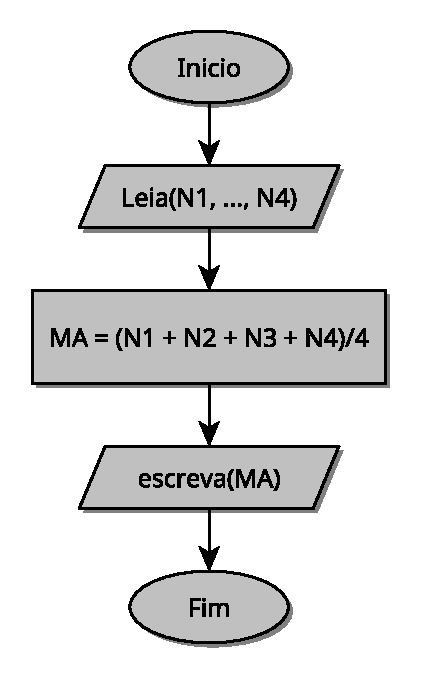
\includegraphics[scale=0.4]{./figures/media_seq.pdf}
	\end{column}
	
	\begin{column}{0.5\textwidth}  %%<--- here
\begin{python}
# Entrada de dados
n1 = float(input('Digite nota 1: '))
n2 = float(input('Digite nota 2: '))
n3 = float(input('Digite nota 3: '))
n4 = float(input('Digite nota 4: '))

# Processamento
ma = (n1 + n2 + n3 + n4)/4

# Saída de dados
print('Média é: ' + str(ma))
\end{python}  
\end{column}
\end{columns}
\end{frame}

\section{Estrutura de decisão}

\begin{frame}[fragile]
\frametitle{Estrutura de decisão}
\small
\vfill \begin{block}{}
 Permite a escolha de um grupo de ações a ser executado quando determinadas condições são satisfeitas.
\end{block}


\begin{itemize}
 \scriptsize
 \vfill \item Simples:
 
 \textbf{if .. :} Se .. :
 
 
 \vfill \item Composto:
 
 \textbf{if .. : .. else:}  Se .. :  senão .. :
 
 \vfill \item Aninhado ou encadeado
 
 \textbf{if .. :} \\
 \hspace{1cm} \textbf{if .. :} \\
 \hspace{2cm} \textbf{if .. :} \\ 
 \hspace{2cm} \textbf{else} \\
%  \hspace{2cm} \textbf{endif} \\
%  \hspace{1cm} \textbf{endif} \\
%  \textbf{endif}
 
\end{itemize}
\end{frame}

\begin{frame}[fragile]
\frametitle{Estrutura de decisão -- simples}

\begin{algorithm}[H]
\scriptsize
\DontPrintSemicolon
\KwData{Notas: $N1, N2, N3, N4$}
\KwResult{Situação do aluno}
\BlankLine
\tcp{Declaração de variáveis}
$N1, N2, N3, N4, MA \gets 0$\;
\BlankLine
\tcp{Entrada de dados}
$N1 \gets \text{leia()}$\;
$N2 \gets \text{leia()}$\;
$N3 \gets \text{leia()}$\;
$N4 \gets \text{leia()}$\;
\BlankLine
\tcp{Processamento}
$MA \gets (N1 + N2 + N3 + N4) / 4$\;
\BlankLine
\tcp{Decisão}
\If{$MA < 6$}{
    $\text{escreva}(\text{Em recuperação})$\;
}
\caption{Decisão simples: média aritmética}
\label{alg:decisao-simples}
\end{algorithm}
\end{frame}



\begin{frame}[fragile]
\frametitle{Estrutura de decisão -- simples}

\begin{columns}
	\begin{column}{0.5\textwidth}		
		\center 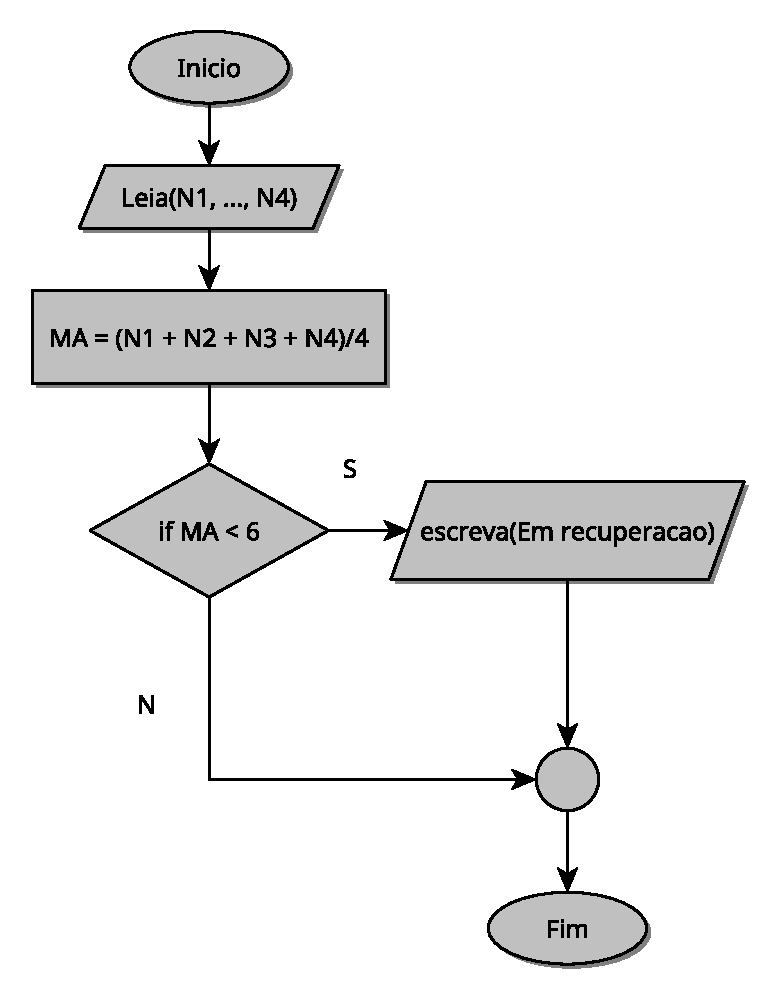
\includegraphics[scale=0.4]{./figures/media-if-simple.pdf}
	\end{column}
	
	\begin{column}{0.5\textwidth}  %%<--- here
\begin{python}
# Entrada de dados
n1 = float(input('Digite nota 1: '))
n2 = float(input('Digite nota 2: '))
n3 = float(input('Digite nota 3: '))
n4 = float(input('Digite nota 4: '))

# Processamento
ma = (n1 + n2 + n3 + n4)/4

# Saída de dados condicionada
if (ma < 6):
    print('Em Recuperação, média é: ' + str(ma))
\end{python}  
	\end{column}
\end{columns}
\end{frame}

\begin{frame}[fragile]
\frametitle{Estrutura de decisão -- composta}

\begin{algorithm}[H]
\scriptsize
\DontPrintSemicolon
\KwData{Notas: $N1, N2, N3, N4$}
\KwResult{Situação do aluno}
\BlankLine
\tcp{Declaração de variáveis}
$N1, N2, N3, N4, MA \gets 0$\;
\BlankLine
\tcp{Entrada de dados}
$N1 \gets \text{leia()}$\;
$N2 \gets \text{leia()}$\;
$N3 \gets \text{leia()}$\;
$N4 \gets \text{leia()}$\;
\BlankLine
\tcp{Processamento}
$MA \gets (N1 + N2 + N3 + N4) / 4$\;
\BlankLine
\tcp{Decisão}
\eIf{$MA < 6$}{
    $\text{escreva}(\text{Em recuperação})$\;
}{
    $\text{escreva}(\text{Aprovado})$\;
}
\caption{Decisão composta: média aritmética}
\label{alg:decisao-composta}
\end{algorithm}
\end{frame}

\begin{frame}[fragile]
\frametitle{Estrutura de decisão -- composta}


\begin{columns}
	\begin{column}{0.5\textwidth}	
	\center 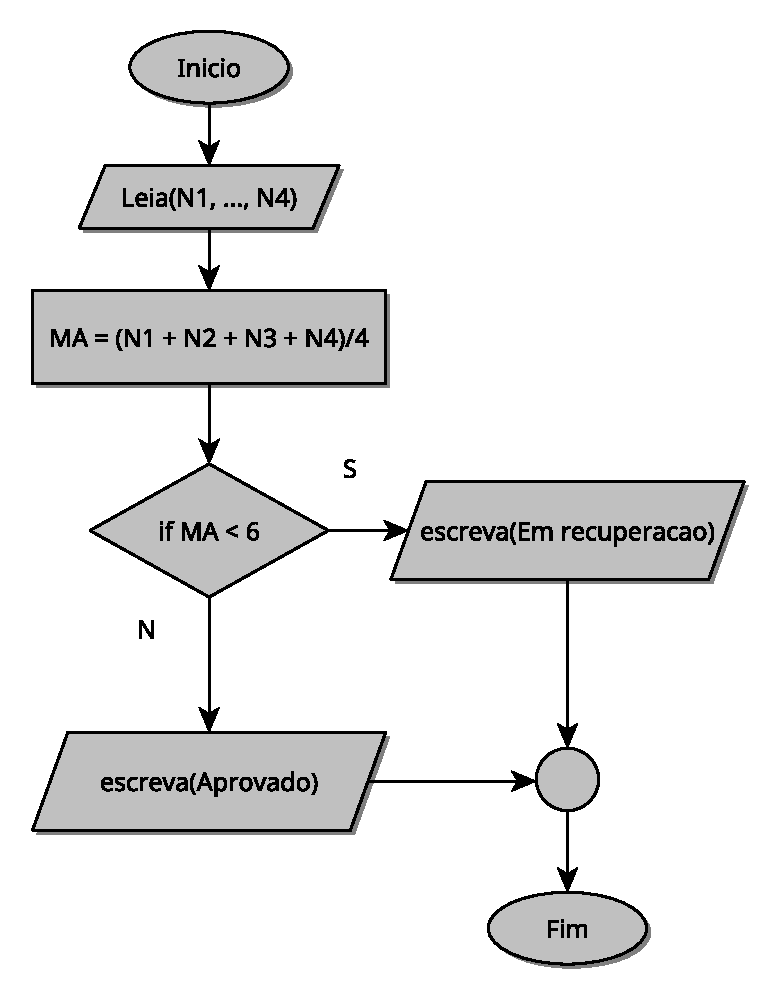
\includegraphics[scale=0.4]{./figures/media-if.pdf}	
	\end{column}
	
\begin{column}{0.5\textwidth}  %%<--- here
\begin{python}
# Entrada de dados
n1 = float(input('Digite nota 1: '))
n2 = float(input('Digite nota 2: '))
n3 = float(input('Digite nota 3: '))
n4 = float(input('Digite nota 4: '))

# Processamento
ma = (n1 + n2 + n3 + n4)/4

# Saída de dados condicionada
if (ma < 6):
    print('Em Recuperação, média é: '  + str(ma))
else:
    print('Aprovado, média é: ' + str(ma))
\end{python}  
\end{column}
\end{columns}
\end{frame}

\begin{frame}[fragile]
\frametitle{Estrutura de decisão -- aninhada}

\begin{columns}
	\begin{column}{0.5\textwidth}	
	\center 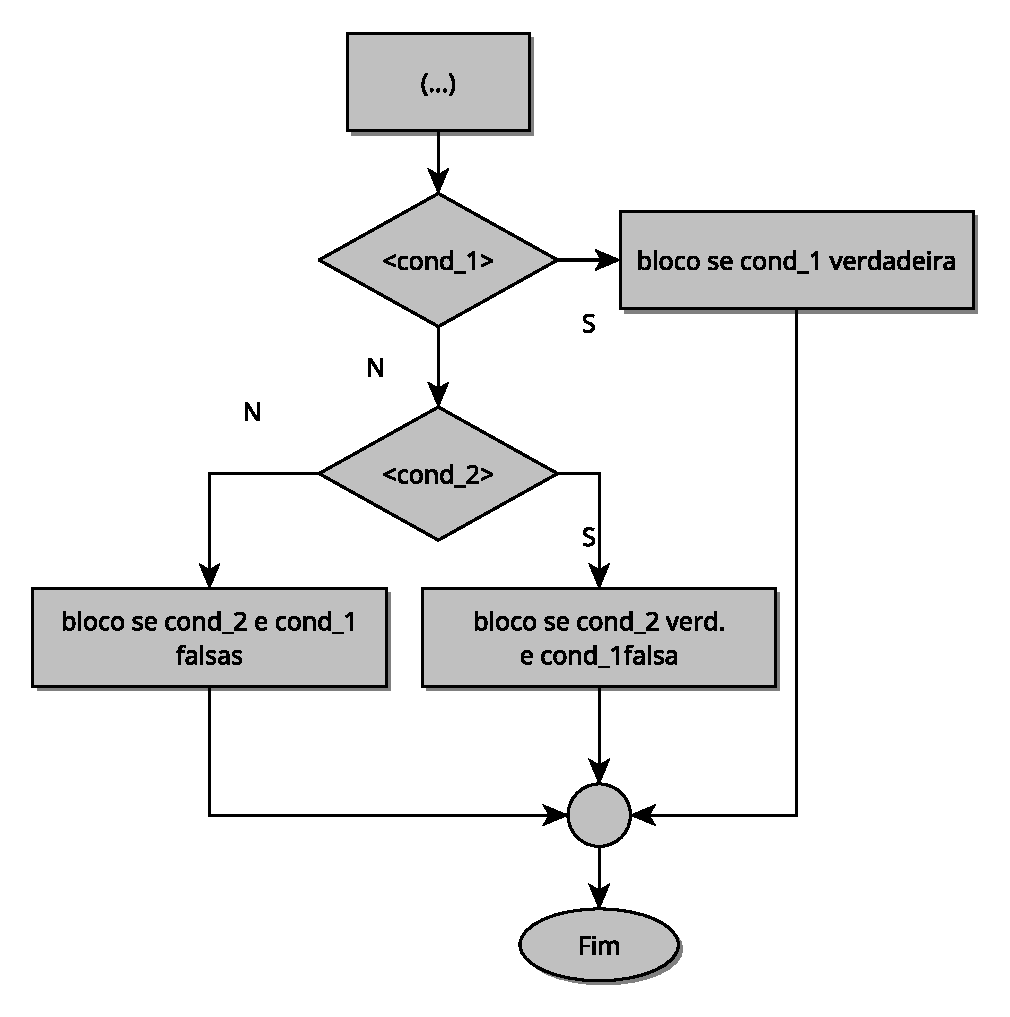
\includegraphics[scale=0.35]{./figures/if-nested.pdf}
	\end{column}

\begin{column}{0.5\textwidth}  %%<--- here
\begin{python}
# Entrada de dados
n1 = float(input('Digite nota 1: '))
n2 = float(input('Digite nota 2: '))
n3 = float(input('Digite nota 3: '))
n4 = float(input('Digite nota 4: '))

# Processamento
ma = (n1 + n2 + n3 + n4)/4

# Saída de dados condicionada
if (ma < 6):
    print('Em Recuperação, média é: ' + str(ma))
else:
    print('Aprovado, média é: ' + str(ma))
    
    if (ma > 9):
        print('Sua media foi maior que 9.')
\end{python}  
\end{column}
\end{columns}
\end{frame}


\begin{frame}[fragile]
 \frametitle{Várias condições}
 
 \begin{itemize}
  \vfill \item Caso houver mais testes, pode-se utilizar a instrução \textbf{elif:}
 \end{itemize}

  
\vfill \begin{python}
temperatura = int(input("Qual a temperatura lá fora? "))

if temperature > 40:
    print("Está quente lá fora")
elif temperature < 15:          # Aqui há um novo teste!
    print("Está frio lá fora")
else:
    print("Está agradável")
    
print("Feito!")
\end{python} 
\end{frame}




\begin{frame}[fragile]
\frametitle{Indentação}

\begin{itemize}
 \vfill \item \textbf{Indentação importa}. Cada linha do \textcolor{red}{if} que é indentada somente será executada se o teste for verdadeiro.
\end{itemize}

\vfill \begin{python}
# Esse código não é válido
if a == 1:
  print("Indentado com 3 espaços.")
    print("Indentado com 4 três espaçoes. Aqui gera erro.")
   print("O computador vai querer que você decida.")

# Quando executado ----------------------------------------------------   
File "<ipython-input-2-b72e5263e892>", line 4
    print("Indentado com 4 três espaçoes. Aqui gera erro.")
    ^
IndentationError: unexpected indent   
\end{python}
\end{frame}

\begin{frame}{Exercícios}
 \begin{center}
  
\includegraphics[scale=0.8]{./figures/man_at_work.png}
 \end{center}
\end{frame}













% \section{Estrutura de decisão}

% \begin{frame}[fragile]
% \frametitle{Estrutura de decisão}
% \small
% \vfill \begin{block}{}
%  Permite a escolha de um grupo de ações a ser executado quando determinadas condições são satisfeitas.
% \end{block}


% \begin{itemize}
%  \scriptsize
%  \vfill \item Simples:
 
%  \textbf{if .. :} Se .. :
 
 
%  \vfill \item Composto:
 
%  \textbf{if .. : .. else:}  Se .. :  senão .. :
 
%  \vfill \item Aninhado ou encadeado
 
%  \textbf{if .. :} \\
%  \hspace{1cm} \textbf{if .. :} \\
%  \hspace{2cm} \textbf{if .. :} \\ 
%  \hspace{2cm} \textbf{else} \\
% %  \hspace{2cm} \textbf{endif} \\
% %  \hspace{1cm} \textbf{endif} \\
% %  \textbf{endif}
 
% \end{itemize}
% \end{frame}

% \begin{frame}[fragile]
% \frametitle{Estrutura de decisão -- simples}

% \begin{algorithm}[H]
% \SetAlFnt{\scriptsize}
% \SetAlCapFnt{\small}
% \DontPrintSemicolon
% \KwData{Notas: $N1, N2, N3, N4$}
% \KwResult{Situação do aluno}
% \BlankLine
% \tcp{Declaração de variáveis}
% $N1, N2, N3, N4, MA \gets 0$\;
% \BlankLine
% \tcp{Entrada de dados}
% $N1 \gets \text{leia()}$\;
% $N2 \gets \text{leia()}$\;
% $N3 \gets \text{leia()}$\;
% $N4 \gets \text{leia()}$\;
% \BlankLine
% \tcp{Processamento}
% $MA \gets (N1 + N2 + N3 + N4) / 4$\;
% \BlankLine
% \tcp{Decisão}
% \If{$MA < 6$}{
%     $\text{escreva}(\text{Em recuperação})$\;
% }
% \caption{Decisão simples: média aritmética}
% \label{alg:decisao-simples}
% \end{algorithm}
% \end{frame}



% \begin{frame}[fragile]
% \frametitle{Estrutura de decisão -- simples}

% \begin{columns}
% 	\begin{column}{0.5\textwidth}		
% 		\center 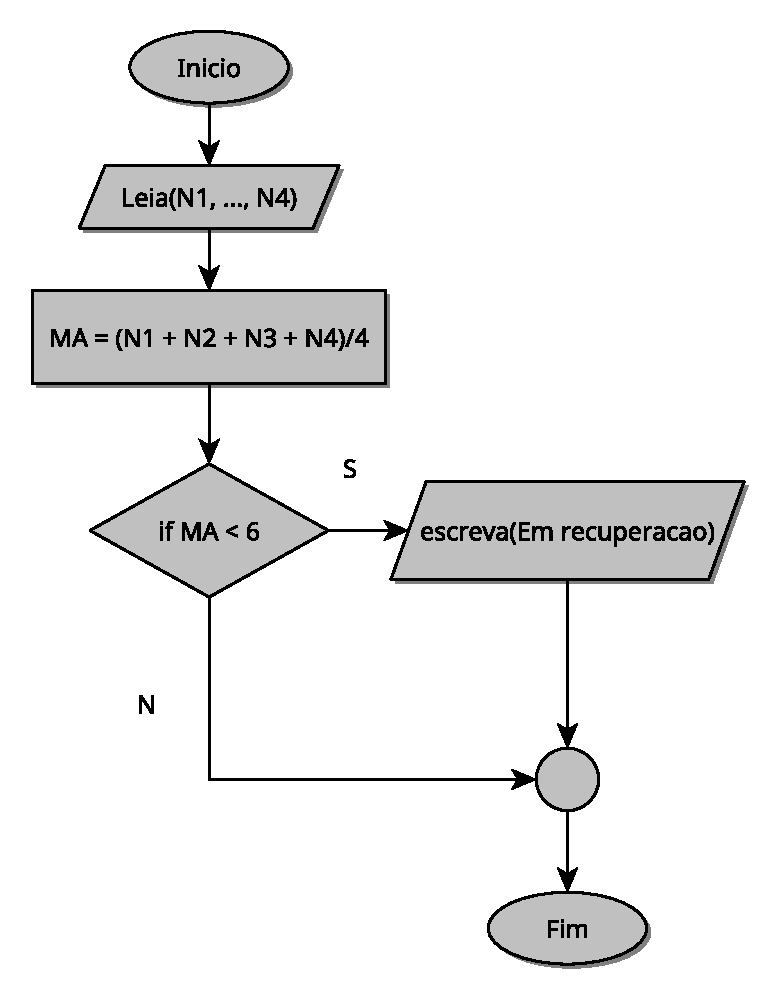
\includegraphics[scale=0.4]{./figures/media-if-simple.pdf}
% 	\end{column}
	
% 	\begin{column}{0.5\textwidth}  %%<--- here
% \begin{python}
% # Entrada de dados
% n1 = float(input('Digite nota 1: '))
% n2 = float(input('Digite nota 2: '))
% n3 = float(input('Digite nota 3: '))
% n4 = float(input('Digite nota 4: '))

% # Processamento
% ma = (n1 + n2 + n3 + n4)/4

% # Saída de dados condicionada
% if (ma < 6):
%     print('Em Recuperação, média é: ' + str(ma))
% \end{python}  
% 	\end{column}
% \end{columns}
% \end{frame}

% \begin{frame}[fragile]
% \frametitle{Estrutura de decisão -- composta}

% \begin{algorithm}[H]
% \SetAlFnt{\scriptsize}
% \SetAlCapFnt{\small}
% \DontPrintSemicolon
% \KwData{Notas: $N1, N2, N3, N4$}
% \KwResult{Situação do aluno}
% \BlankLine
% \tcp{Declaração de variáveis}
% $N1, N2, N3, N4, MA \gets 0$\;
% \BlankLine
% \tcp{Entrada de dados}
% $N1 \gets \text{leia()}$\;
% $N2 \gets \text{leia()}$\;
% $N3 \gets \text{leia()}$\;
% $N4 \gets \text{leia()}$\;
% \BlankLine
% \tcp{Processamento}
% $MA \gets (N1 + N2 + N3 + N4) / 4$\;
% \BlankLine
% \tcp{Decisão}
% \eIf{$MA < 6$}{
%     $\text{escreva}(\text{Em recuperação})$\;
% }{
%     $\text{escreva}(\text{Aprovado})$\;
% }
% \caption{Decisão composta: média aritmética}
% \label{alg:decisao-composta}
% \end{algorithm}
% \end{frame}

% \begin{frame}[fragile]
% \frametitle{Estrutura de decisão}


% \begin{columns}
% 	\begin{column}{0.5\textwidth}	
% 	\center 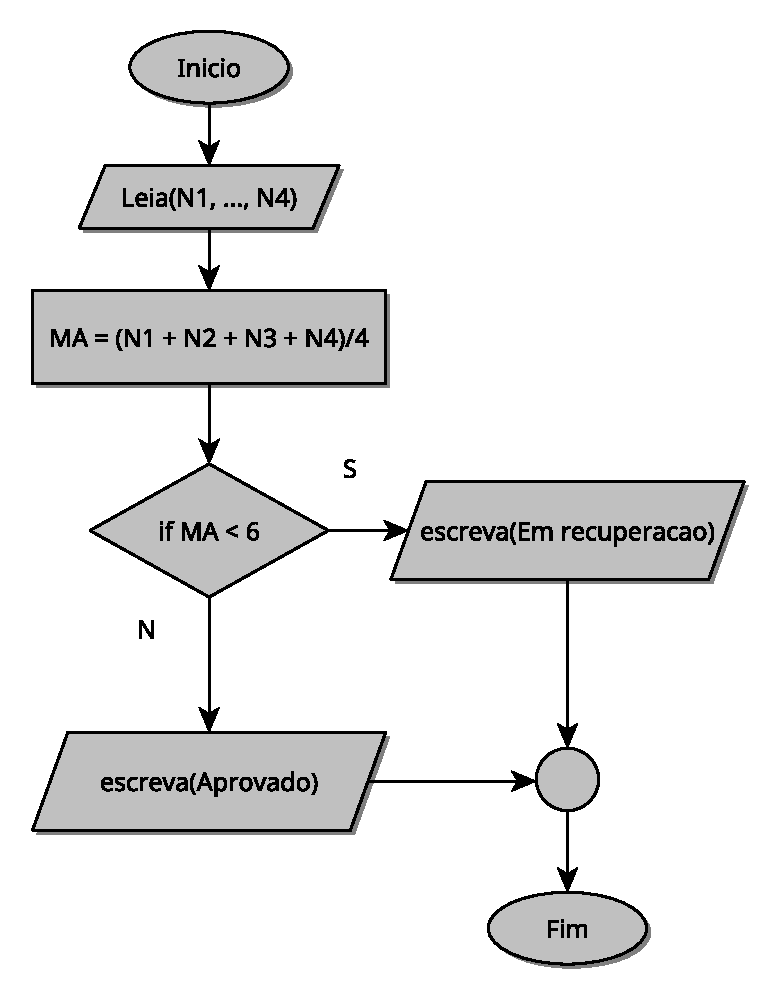
\includegraphics[scale=0.4]{./figures/media-if.pdf}	
% 	\end{column}
	
% \begin{column}{0.5\textwidth}  %%<--- here
% \begin{python}
% # Entrada de dados
% n1 = float(input('Digite nota 1: '))
% n2 = float(input('Digite nota 2: '))
% n3 = float(input('Digite nota 3: '))
% n4 = float(input('Digite nota 4: '))

% # Processamento
% ma = (n1 + n2 + n3 + n4)/4

% # Saída de dados condicionada
% if (ma < 6):
%     print('Em Recuperação, média é: '+ str(ma))
% else:
%     print('Aprovado, média é: ' + str(ma))
% \end{python}  
% \end{column}
% \end{columns}
% \end{frame}


% \begin{frame}[fragile]
%  \frametitle{Várias condições}
 
%  \begin{itemize}
%   \vfill \item Caso houver mais testes, pode-se utilizar a instrução \textbf{elif:}
%  \end{itemize}

  
% \vfill \begin{python}
% temperatura = int(input("Qual a temperatura lá fora? "))

% if temperature > 40:
%     print("Está quente lá fora")
% elif temperature < 15:          # Aqui há um novo teste!
%     print("Está frio lá fora")
% else:
%     print("Está agradável")
    
% print("Feito!")
% \end{python} 
% \end{frame}


\section{Estrutura de repetição}

\begin{frame}[fragile]
\frametitle{Estrutura de repetição}
\small

\vfill \begin{block}{}
 \textbf{Permite repetir um grupo de ações enquanto determinadas condições são satisfeitas.}
\end{block}

\begin{itemize}
 \vfill \item Denominados laços ou \textit{loops}
 \small
 
 \vfill Tipos básicos:
 
 \begin{itemize}
    \small
    \vfill \item enquanto: \textbf{while}
  
    \vfill \item para: \textbf{for}
  
 \end{itemize}
 
 \vfill\item Todas estas estruturas podem ser aninhadas, ou seja, \textbf{while} contendo outro \textbf{while}, \textbf{while} contendo um ou vários \textbf{for}, ...

 
\end{itemize}
\end{frame}



\section{Enquanto -- while}


\begin{frame}
 \frametitle{Enquanto -- while}
 
 \begin{itemize}
    \vfill \item Teste lógico no \textbf{início do laço}
  
    \vfill \item Executa repetição \textbf{enquanto} a condição for verdadeira 
 \end{itemize}
 
 \vfill \center 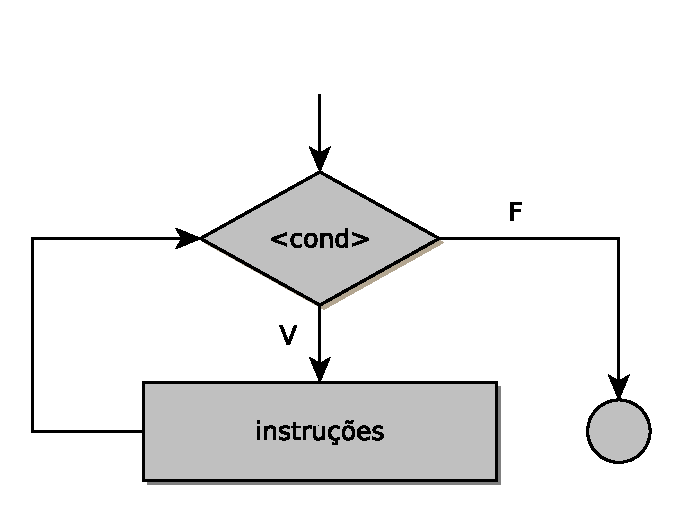
\includegraphics[scale=0.5]{./figures/while-simple.pdf}
 
\end{frame}

\begin{frame}[fragile]
\frametitle{Média para 10 Alunos}
\tiny
\begin{algorithm}[H]
\SetAlFnt{\tiny}
\SetAlCapFnt{\tiny}
\DontPrintSemicolon
\KwData{Notas de 10 alunos}
\KwResult{Situação de cada aluno}
\BlankLine
\tcp{Declaração de variáveis}
$N1, N2, N3, N4, MA \gets 0$\;
$CONTADOR \gets 0$\;
\BlankLine
\tcp{Laço de repetição}
\While{$CONTADOR < 10$}{
    \tcp{Entrada de dados}
    $N1 \gets \text{leia()}$\;
    $N2 \gets \text{leia()}$\;
    $N3 \gets \text{leia()}$\;
    $N4 \gets \text{leia()}$\;
    \BlankLine
    \tcp{Processamento}
    $MA \gets (N1 + N2 + N3 + N4) / 4$\;
    \BlankLine
    \tcp{Decisão}
    \eIf{$MA < 6$}{
        $\text{escreva}(\text{Em recuperação})$\;
    }{
        $\text{escreva}(\text{Aprovado})$\;
    }
    $CONTADOR \gets CONTADOR + 1$\;
}
\caption{Cálculo de média para 10 alunos}
\label{alg:media-10-alunos}
\end{algorithm}
\end{frame}



\begin{frame}[fragile]
\frametitle{Estrutura de repetição: while}

\begin{columns}
    \begin{column}{0.5\textwidth}	
    \center 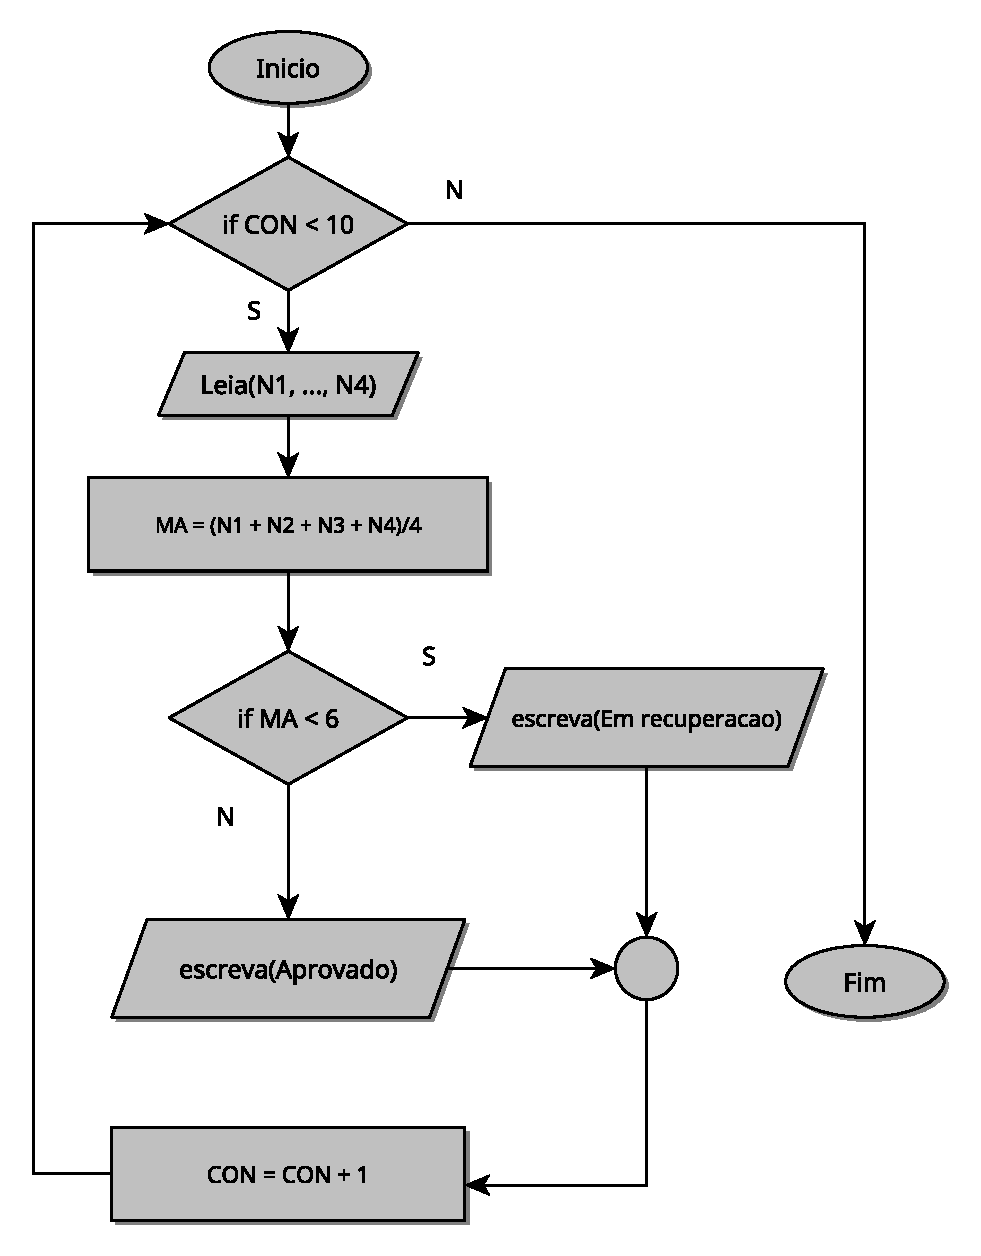
\includegraphics[scale=0.3]{./figures/while-media.pdf}	
    \end{column}
    
\begin{column}{0.5\textwidth}  %%<--- here
\begin{python}
# Variável de contagem (condição do while)
contador = 0

# Repetição
while (contador < 10):
    print('Aluno: ' + str(contador))
    
    # Entrada de dados
    n1 = float(input('Digite nota 1: '))
    n2 = float(input('Digite nota 2: '))
    n3 = float(input('Digite nota 3: '))
    n4 = float(input('Digite nota 4: '))

    # Processamento
    ma = (n1 + n2 + n3 + n4) / 4
    
    # Decisão
    if ma < 6:
        print('Em recuperação: ' + str(ma))
    else:
        print('Aprovado: ' + str(ma))
    
    # Contador de alunos
    contador = contador + 1

# Fim do while (indentado à direita)
print('Cálculos concluídos')
\end{python}  
\end{column}
\end{columns}
\end{frame}


\begin{frame}[fragile]
    \frametitle{Estrutura de repetição: while}

\begin{python}
# Continuação (condição do while)
continuar = 's'

# Repetição
while (continuar == 's'):
    
    # Entrada de dados
    n1 = float(input('Digite nota 1: '))
    n2 = float(input('Digite nota 2: '))
    n3 = float(input('Digite nota 3: '))
    n4 = float(input('Digite nota 4: '))

    # Processamento
    ma = (n1 + n2 + n3 + n4) / 4
    
    # Decisão
    if ma < 6:
        print('Em recuperação: ' + str(ma))
    else:
        print('Aprovado: ' + str(ma))

    # Continuar ou não?
    continuar = input('Deseja continuar (s/n): ')

# Fim do while (indentado à direita)
print('Cálculos concluídos')
\end{python}  
\end{frame}   

\section{Para -- for}

\begin{frame}
    \frametitle{Estrutura de repetição: for}
 
    \vspace{-1cm}

    \vfill\begin{block}{}
    Laços \textbf{for} são utilizados para iterar em uma sequência. 
    \end{block}

    \vfill \begin{itemize}
    \item Em cada iteração, a variável definida no laço irá incrementar.
    \end{itemize}

    \vfill \center 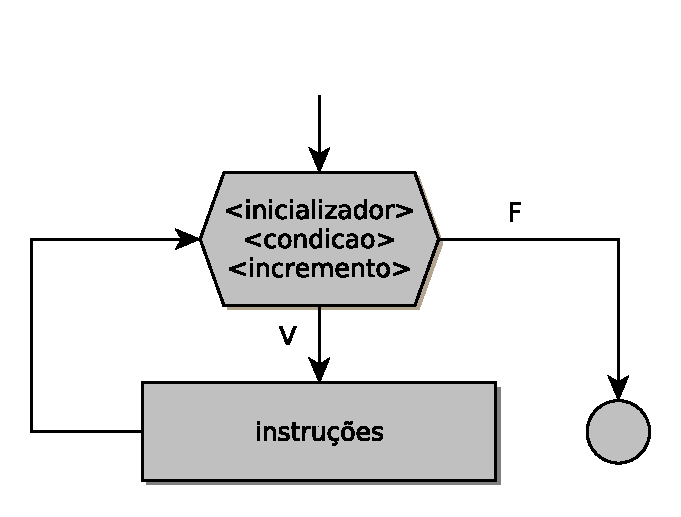
\includegraphics[scale=0.35]{./figures/for-simple.pdf}
 
\end{frame}


\begin{frame}[fragile]
    \frametitle{Estrutura de repetição: for}

Strings são sequências de caracteres:
\begin{python}
# Para cada letra em "banana"
for letra in "banana":
  print(letra)
\end{python}

Saída: 

\begin{python}
b
a
n
a
n
a
\end{python}
\end{frame}   

\begin{frame}[fragile]
    \frametitle{Estrutura de repetição: for}

\begin{python}
# Para cada letra em "banana"
for letra in "banana":
    if letra == 'a':
        print('A')
    else:
        print(letra) 
\end{python}

Saída: 

\begin{python}
b
A
n
A
n
A
\end{python}
\end{frame}   


\begin{frame}[fragile]
    \frametitle{Estrutura de repetição: sequências numéricas}

\begin{python}
# Para uma sequência de 6 números: [0,6[
for numero in range(6):
    print(numero)
\end{python}

Saída: 

\begin{python}
0
1
2
3
4
5
\end{python}
\end{frame} 


\begin{frame}[fragile]
    \frametitle{Sequências numéricas: função range}

\begin{python}
# Range começa em 0 por padrão:
for numero in range(6):     # Intervalo [0,5] ou [0,6[


# Range pode começar em 2 até 10, mas 10 não é incluso
for numero in range(2,10):     # Intervalo [2,10[


# Para mudar o intervalo de incremento
for numero in range(2,30,3):     # Intervalo [2,30[ 
                                 # com incremento de 3

\end{python}

\begin{itemize}
    \item range(início, fim, incremento)
\end{itemize}

\end{frame} 

\begin{frame}[fragile]
    \frametitle{Sequências numéricas: tabuada}

\begin{python}
# Pede para o usuário
tabuada = int(input('Qual tabuada? '))

print('Range(0,11)')
for numero in range(0,11):
    print(numero * tabuada)
    
# ou
print('Range mais esperto')
for numero in range(0, tabuada * 11, tabuada):
    print(numero)
\end{python}

\end{frame} 





\begin{frame}[fragile]
    \frametitle{Sequências numéricas: funções matemáticas}

\begin{python}
# Valores de uma parábola

for x in range(-10,11):
    y = x**2 -9*x + 2
    print(y)
    
\end{python}
\begin{python}
192		      -16
164		      -18
138		      -18
114		      -16
92 		      -12
72 		       -6
54 		       2
38 		      12
24 		      
12 		      
2 		      
-6		      
-12		      
\end{python}

\end{frame} 



\begin{frame}[fragile]
\frametitle{Indentação}

\begin{itemize}
 \vfill \item \textbf{Indentação importa}. Cada linha do \textcolor{red}{for/while} que é indentada somente será executada se o teste for verdadeiro.
\end{itemize}

\vfill \begin{python}
# Esse código não é válido
while (a == 1):
  print("Indentado com 3 espaços.")
    print("Indentado com 4 três espaçoes. Aqui gera erro.")
   print("O computador vai querer que você decida.")

# Quando executado ----------------------------------------------------   
File "<ipython-input-2-b72e5263e892>", line 4
    print("Indentado com 4 três espaçoes. Aqui gera erro.")
    ^
IndentationError: unexpected indent   
\end{python}
\end{frame}

\begin{frame}{Exercícios}
 \begin{center}
  
\includegraphics[scale=0.8]{./figures/man_at_work.png}
 \end{center}
\end{frame}


\end{document}


% 
%
% Local variables section, for Emacs: specifies that this file is the main one.
%
%
%%% Local Variables:
%%% TeX-master: t
%%% End:
